
\chapter{Theoretical Motivation}
\label{chap:motivation}
\section{The Standard Model}

\indent  The standard model (SM) describes our current understanding of the interactions of all known elementary particles.  SM is composed of 3 parts; fermions with spin 1/2 that make up the visible matter in our universe; vector bosons with spin 1 that mediates the interactions between the fermions; and a scalar spin 0 Higgs boson that gives mass to the massive fermions and the $W$ and $Z$ vector bosons.  The fermions are organized in two groups, the quarks and leptons, with three families of increasing mass.  The force mediators, the photon, $W/Z$ boson, and gluon are respectively responsible for the electromagnetic, weak, and strong interactions.  A diagram displaying the SM particles is shown in figure \ref{fig:SM:part}. \\

\begin{figure}[htbp]
	\begin{center}
		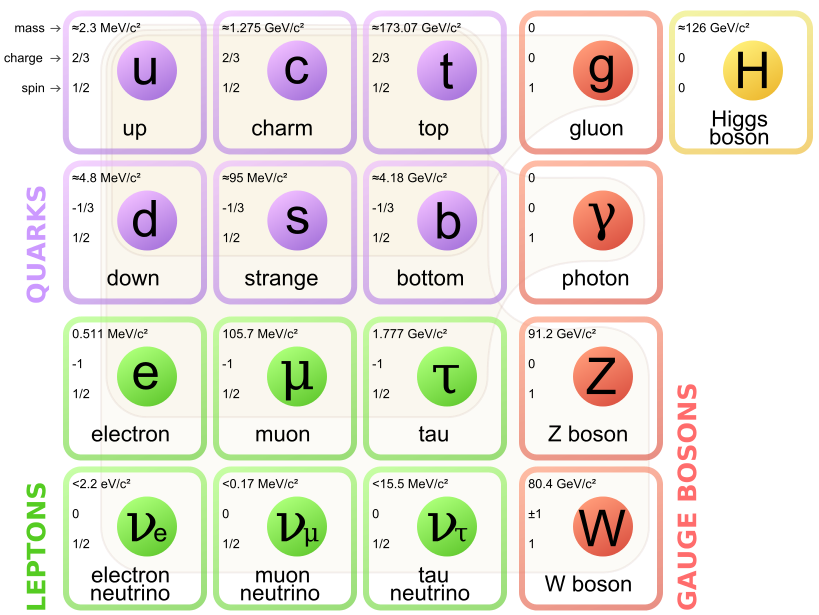
\includegraphics[width=0.85\textwidth]{figures/theory/Standard_Model_of_Elementary_Particles.png}
		\caption{List of standard model elementary particles}
		\label{fig:SM:part}
	\end{center}
\end{figure}

\indent  Interactions in the SM are described by non-abelian Yang-Mills gauge theory with the gauge group $SU(3)_C \times SU(2)_L \times U(1)_Y$ where $SU(3)_C$ corresponds to the strong interaction and $SU(2)_L \times U(1)_Y$ corresponds to the electroweak interactions. 

\indent The quarks can interact via the strong interaction described by the $SU(3)_C$ symmetry.  These quarks carry color charge in addition to their electromagnetic charges.  The gluons mediate the strong interactions but unlike electrically neutral photons, gluons carry color charge.  The self interaction of the gluon causes the coupling strength of the strong coupling constant $\alpha_s$ to diverge at low energies.  This phenomena, called confinement, ensures that quarks are confined to be within composite color singlet states in the form of hadrons.  At the same time, the running of $\alpha_s$ approaches zero at high energy; forming a phenomenon known as asymptotic freedom. \\

\indent For energetic particles like those produced in proton-proton collisions at the LHC, colored partons will recursively radiate collinear gluons and quark/anti-quark pairs in a parton shower. These partons eventually form color-singlet hadrons once the energy scale is lower then IR-cutoff scale due to confinement.  The result is a jet of color-neutral baryons and mesons localized in a narrow cone in the direction of the initial colored parton. \\

\indent Both quarks and leptons also interact via the weak interaction.  Specifically, the left handed component of the fermions form an $SU(2)_L$ doublet while the right handed handed components form an $SU(2)_L$ singlet.  Therefore, only the left handed components of SM fermions carry weak charge and interact via the weak interaction.  \\

\indent The generators of the gauge groups correspond to the massless spin one vector bosons.  The $W^\pm$ and $Z$ bosons acquire mass through spontaneous electroweak symmetry breaking using the Higgs mechanism.  This is accomplished using an additional $SU(2)_L$ doublet of complex spin zero fields, the Higgs field.  The Higgs has a nonzero vacuum expectation value (VEV) at the minimum of its quadratic potential shown in equation \ref{eqn:Higgs}.  When $\lambda > 0$ and $m_H^2 < 0 $, $\braket{H} = \sqrt{-m_H^2/2\lambda}$.  \\

\begin{equation}
\label{eqn:Higgs}
V(H) = m_H^2 |H|^2 +\lambda |H|^4
\end{equation}

\indent This breaks the $SU(2)_L \times U(1)_Y$ electroweak symmetry and leaves only the $U(1)_{em}$ electromagnetism invariant.  Meanwhile, the other gauge bosons from $SU(2)_L \times U(1)_Y$ gains a longitudinal degree of freedom from degrees of freedom associated with the Higgs doublet and thereby gaining mass.  The photon, $W^\pm$ and $Z$ bosons are therefore linear combinations of the original $SU(2)_L and U(1)_Y$ generators.  The Higgs boson also gives fermions their mass through Yukawa couplings. \\

\indent After symmetry breaking, only one neutral scalar component of the Higgs doublet is left.  This is the massive Higgs boson observed in July 2012 at the LHC.  \\

\section{Introduction to Super-Symmetry}
\label{Theory:QFT}

%\indent Current combined measurement of the Higgs boson at ATLAS and CMS gives an observed Higgs mass of $125.09\pm0.21$(stat)$\pm0.11$(syst) GeV.\cite{Higgs2016}  Plus $\braket{H} \sim 174 \gev$ due to experimental measurements of the properties of the weak interactions.  This implies that the parameters $\lambda$ and $m_H^2$ in the Higgs potential in equation \ref{eqn:Higgs} have the values of $0.126$ and $-(92.9 \gev)^2$ assuming SM is the correct effective field theory.  \\

\indent Theoretical calculations of the self interaction of the Higgs field give enormous quantum corrections to $m_H^2$.\cite{MartinSUSY}  For example, the correction to $m_H^2$ from a loop containing a Dirac fermion $f$ with mass $m_f$ is given in equation \ref{eqn:Higgs:Loopf}.  The Feynman diagram associated with the fermion loop is shown in figure \ref{fig:Higgs:Loopf} \\

\begin{equation}
\label{eqn:Higgs:Loopf}
\Delta m_H^2 = - \frac{|\lambda_f|^2}{8\pi^2}\Lambda^2_{UV} + ....
\end{equation}

\begin{figure}[htbp]
	\begin{center}
		\includegraphics[width=0.45\textwidth]{figures/theory/loopf.png}
		\includegraphics[width=0.45\textwidth]{figures/theory/loopS.png}
		\caption{One-Loop corrections due to a Dirac fermion $f$ and a scalar $\tilde{f}$ to the Higgs mass parameter $m_H^2$}
		\label{fig:SM:Loopf}
	\end{center}
\end{figure}

\indent $\lambda_f$ is the Yukawa coupling between the fermion and the Higgs and $\Lambda_{UV}$ is the ultraviolet cutoff used to regulate the loop integral.  $\Lambda_{UV}$ can be interpreted as around the energy scale of new physics.  Since the scale of new physics maybe orders of magnitudes larger then the electroweak scale, the quadratic dependence of $m_H^2$ on $\Lambda_{UV}$ makes the Higgs potential extremely sensitive to new physics. This sensitivity to high mass scales for the Higgs potential is referred to as the hierarchy problem.  \\ %Additional terms also exists in the correction but they grow at most logarithmically in $\Lambda_{UV}$. \\

\indent Supersymmetry (SUSY) solves this problem by proposing that there exist a new space-time symmetry with respect to the transformation $Q$ that turns fermions into bosons and bosons into fermions.\\

\begin{equation}
\label{eqn:Higgs:Loopf}
Q\ket{Boson} = \ket{Fermion} ~~~~~~~~~~~~~~~~~~~~~~~~~~~~ Q\ket{Fermion} = \ket{Boson}
\end{equation}

\indent The supersymmetric Lagrangian is invariant under transformations of $Q$ and $Q^{\dagger}$.  In order for this to be satisfied, SUSY proposes the existence of a supersymmetric partner (superpartner) to every known SM particle.  SM particles and their superpartners are related to each other by the Q transformation and differ from each other by spin $1/2$.  If SUSY was an exact symmetry then the SM particle and its superpartner must have the same mass.  However, we have yet to discover even a single superpartner to the SM at collider experiments.  Therefore, SUSY must be broken at low energies and the superpartners have significantly more mass then their SM counter parts.  \\

\indent Supersymmetry breaking can occur in many ways; the details of which are beyond the scope of this thesis.  More details on SUSY symmetry breaking can be found in \cite{MartinSUSY}.  A brief summary of one example of supersymmetry break called Gauge-mediated supersymmetry breaking (GMSB) will be given here.   In GMSB, some scalar fields in the SUSY Lagrangian gains a vacuum expectation value due to their potential energy shape.  This symmetry breaking gives mass to some fermions and their super-partners called messengers.  Both the scalars and the messengers are too heavy to be directly detectable and are not the SM superpartners.  \\

\indent Instead, the messengers contribute effective mass to the superpartners of SM particles via loop interactions.  Gauge symmetry ensures that the loop correction to the SM gauge bosons are zero to all orders of magnitudes, but the same protection is not afforded to their superpartners, the gauginos.  These gauginos gain effective mass through one-loop diagrams involving virtual messenger particles.  In a similar fashion, the scalar partners to SM fermions gain effective mass through two-loop diagrams involving virtual messengers and SM gauge bosons.  In these way, GMSB leads to heavier superpartners relative to their SM counter parts.  \\

%\indent For the purpose of this document, we will only look at the phenomenological consequences of heavy superpartners and not be concerned with the exact SUSY breaking method.  \\

\indent In general, if a complex scalar particle $\tilde{f}$~with mass $m_{\tilde{f}}$~exists and couples to the Higgs according to the term $-\lambda_S|H|^2|\tilde{f}|^2$ then correction to the Higgs mass due to the loop diagram in figure \ref{fig:SM:Loopf} is given in equation \ref{eqn:Higgs:LoopS}. \\

\begin{equation}
\label{eqn:Higgs:LoopS}
\Delta m_H^2 = \frac{\lambda_s}{16\pi^2}[\Lambda^2_{UV} - 2m_{\tilde{f}}^2 \ln{\Lambda_{UV}/m_{\tilde{f}}}+ ....]
\end{equation}

\indent This correction also contains a quadratically divergent term that has an opposite sign to equation \ref{eqn:Higgs:Loopf}.  The two quadratic contributions to $m_H^2$ will cancel if $|\lambda_f|^2 = \lambda_s$ and we are left with only a term that is proportional to $\ln{\Lambda_{UV}/m_{\tilde{f}}}$. In fact, this cancellation of quadratically divergent term will occur not only for the one loop case, but for all orders of magnitude in perturbation theory if supersymmetry exists. \\

\indent The term that remains after cancellation is proportional to equation \ref{eqn:Higgs:logterm}. \\

\begin{equation}
\label{eqn:Higgs:LoopS}
\Delta m_H^2 \sim m_{\tilde{f}}^2[\frac{\lambda_s}{16\pi^2}\ln{\Lambda_{UV}/m_{\tilde{f}}}]
\end{equation}

\indent Its important to note that while the correction is now not so strongly dependent on $\Lambda_{UV}$ because of the natural log, the correction term is also directly proportional to $m_{\tilde{f}}^2$.  This implies that the superpartners masses cannot be too large, otherwise the correction to $m_H^2$ is again too large.  If we set $\Lambda_{UV}$ to approximately the Planck scale $M_P$ and $\lambda_s \sim 1$, we find that $m_{\tilde{f}}$~for the lightest supersymmetric particle should not be heavier then the $\tev$ scale if we want to avoid any unphysical fine-tuning on the Higgs mass.\cite{MartinSUSY}  \\

\indent In particular, we know that the superpartner to the top quark has a coupling to the Higgs of order $1$ due to $\lambda_S = |\lambda_f|^2 \sim 0.94^2$. This makes searches for the stop especially interesting as it is potentially within reach of the energy of the LHC. \\

\subsection{R-Parity Conservation}

\indent Supersymmetry introduces many new interactions not found in the SM.  Some of these interactions directly violate total lepton and baryon numbers.  If such interactions exist then the half life of a proton may be only a tiny fraction of a second.  However, proton decay experiments have shown that the proton half-life exceeds $10^{32}$ years.  A new discrete symmetry, called R-parity, is introduced to remove these B and L violating terms from the supersymmetric Lagrangian.  \\

\indent The quantity $P_R$ defined in equation \ref{eqn:PR} and must multiply to 1 for all interaction vertexes for R-parity to be conserved. $P_R$ equals $1$ for all SM particles and equals $-1$ for all superpartners.  \\

\begin{equation}
\label{eqn:PR}
P_R = (-1)^{3(B-L)+2s}
\end{equation}

\indent R-parity conservation has several important phenomenological consequences.  In R-parity respecting SUSY, superpartners are always produced in pairs.  Superpartners must always decay into other superpartners forming a long decay chain of SUSY particle to SUSY particle that ultimately end in the lightest supersymmetric particle (LSP) which is absolutely stable.  If the LSP is electrically and color neutral, then it is an attractive dark matter candidate.  \\

\indent In this search, we assume R-parity is conversed and the LSP is a weakly interacting neutralino.  \\
